\Gls{ml} has become an important sub-field of computer science. It emulates human-like learning using mathematical models, so predictions can be made about new data in the future. Rather than explicitly programming how to make those predictions, the developer provides sample data during \textit{training}. Once the accuracy of the trained model is sufficient, it can be used for \textit{inference}. The model can be thought of as the approximation of a function mapping from the input data to some output, e.g., a label for classification, or a numerical value for regression~\cite[p.~164]{IanGoodfellow.2016}.

\section{Artificial Neural Networks}
While there are a variety of \gls{ml} models in use today, \glspl{ann} are among the most powerful and flexible, due to their ability to represent complex functions~\cite[p.~163]{IanGoodfellow.2016}. They find application in fields as diverse as image and speech recognition, movie recommendations and medical diagnosis.

\Glspl{ann} are composed of multiple layers, with the output of one layer being the input of another layer. The first layer receives the input data, and the last layer produces the final output. With an increasing number of layers, or \textit{depth} of the network, more complex functions can be approximated. These deep networks are subject of the \gls{ml} sub-field of \gls{dl}. All layers perform some computation given a set of trained or specified parameters and the input. Both parameters and inputs are tensors, a higher-dimensional generalization of vectors and matrices. Traditional \glspl{ann} feature only fully-connected layers with some activation function.

Grid-like data such as time series (1D) or images (2D) benefit from additional layers found in \glspl{cnn}~\cite[p.~326]{IanGoodfellow.2016}. This makes \glspl{cnn} an important tool in state-of-the-art computer vision applications. \Glspl{cnn} apply convolution and pooling to a region of the input tensor in a sliding fashion, so values only interact with other values that are located in their neighborhood. Convolution applies one or more kernel matrices to the input, which are element-wise multiplied with the current region and then summed up into a single output value. Pooling averages or finds the maximum of the region as output value. Both operations support a variable stride (step size) and padding.

While neural network models logically consist of a series of layers, machine learning frameworks usually represent them in a computation graph. The computation graph's first vertex is the input node, followed by a number of tensor operators with their parameters performing the layer's computations, and finally an output node. The edges describes how data flows between the vertices.

\section{Inference Optimization}
Typically, the amount of inferences heavily outweighs the amount of trainings, since training only needs to be done once (albeit model re-training is usually done periodically when new training data is available). For this reason, while training takes longer by several orders of magnitude, speeding up inference has a larger impact and is a worthwhile endeavor. 
Reduction of the inference time has a number of advantages:
\begin{itemize}
	\item less hardware is required to achieve the same inference rate
	\item a higher inference rate can be achieved with same hardware
	\item real-time applications are facilitated, e.g., autonomous driving, industrial monitoring
\end{itemize}
In real-time applications with a high inference rate, even small improvements in inference performance (in the order of milliseconds) can be critical to guarantee the required throughput.
For example, a major hard drive manufacturer detects defects in their products using a \gls{cnn}-based smart manufacturing solution~\cite[p.~11]{LyveDataLabs.2019}. They perform inference on 3 million images every day, so if they could only save \SI{5}{\milli\second} per image due to some performance optimization, that would amount to over \SI{4}{\hour} less total inference time every day~\cite{Seagate.2019}. Alternatively, they could save costs by needing less servers that are equipped with expensive accelerator devices.

Accelerator devices such as \glspl{gpu}, ASICs like tensor processing units or FPGAs are used to speed up both training and inference. However, generic \gls{ml} models cannot make full use of accelerator capabilities and fall short of leveraging the full potential. Every device has different features such as specialized instructions, memory size and layout, cache access, and parallelization support. This means that models need to be attuned to the \textit{\gls{targetdevice}} to achieve the best inference performance. But even if no special accelerator devices are used but only a conventional CPU, adapting to the specific architecture can yield great performance benefits~\cite[p.~1]{Liu.2019}. In a traditional machine workflow, the trained model is deployed as-is (Figure \ref{fig:ml-workflow-old}). Inference optimization adds an additional step, turning the trained model into a functionally equivalent but optimized version before inference (Figure \ref{fig:ml-workflow-new}). In this step, we first apply high-level transformations that rewrite the computation graph by, for example, fusing tensor operators, pre-computing constant parts or transforming the data layout in memory~\cites[p.~1--3]{Chen.2018b}. More importantly, however, we can change the low-level implementation of tensor operators.

\begin{figure}
	\begin{minipage}[b]{.5\textwidth}
		\centering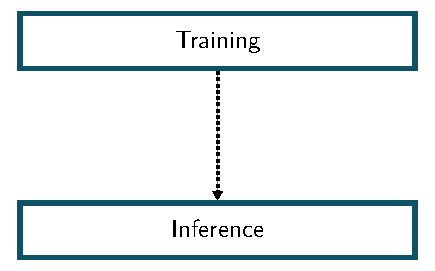
\includegraphics{ml_workflow_1.pdf}
		\subcaption{Traditional without inference optimization}\label{fig:ml-workflow-old}
	\end{minipage}%
	\begin{minipage}[b]{.5\textwidth}
		\centering\includegraphics{ml_workflow_2.pdf}
		\subcaption{Improved with inference optimization}\label{fig:ml-workflow-new}
	\end{minipage}
	\caption[Traditional vs. optimized machine learning workflow]{Machine learning workflow}
	\label{fig:ml-workflow}
\end{figure}

The model determines what tensor operators are calculated, but it does not specify how they are calculated. Deliberately choosing the actual implementation offers great optimization potential. There is always a generic naïve implementation, which is the straightforward way of performing the calculation. However, it does not consider, e.g., memory sharing between threads or cache access patterns, which can have a significant adverse effect on performance~\cite{Hu.2017}. Techniques such as loop unrolling, reordering and tiling as well as multi-dimensional threading and tensor compute instructions can help leverage the accelerator's capabilities, but there is an abundance of combinations of settings for these techniques, the best of which is very much specific to the target device~\cite[p.~2]{Chen.2018b}. Finding the optimal such combination is the key aspect of tensor operator optimization.

Convolution operators are computationally very intensive and make up the majority of modern \glspl{cnn}, such as Inception\cite{Szegedy.2015} and ResNet\cite{He.2015}. Therefore, tensor operator optimization should focus on convolution over other types like pooling and fully-connected. It is not possible to optimize convolutions in general, but we need to optimize for every distinct parameter set that is present in the computation graph, i.e. combination of input shape, kernel shape, padding, and stride. This means that the effort increases with a higher variety of layer configurations.

\section{Manual Optimization}
Optimized implementations for tensor operators with a specific parameter set are provided by accelerator vendors in libraries like cuDNN for NVIDIA \glspl{gpu} and Intel Math Kernel Library for Intel CPUs. The vendors possess the hardware-specific knowledge to write good implementations by hand, but human expertise is required for this approach. While state-of-the-art, manual optimization has a number of inherent shortcomings:
\begin{itemize}
	\item slow support for new devices
	\item slow support for new graph-level optimizations
	\item no support for unconventional shapes
	\item vendor lock-in
\end{itemize}
These limitations hinder innovation, which is undesirable in a field so fast-evolving and relatively young as \gls{dl}. Researchers need to make a choice between avoiding devices, high-level optimizations and new network architectures that are not supported by those predefined operator libraries, and using unoptimized implementations~\cite[p.~1]{Chen.2018b}.

\section{Automated Optimization}
Automated tensor operator optimization, or \textit{autotuning}, overcomes these shortcomings by eliminating the need for human experts. Vendor-agnostic frameworks can discover good implementations regardless of hardware, model or graph optimizations. This enables innovation by fostering experimentation with novel or unconventional layers and high-level transformations that are not supported by manual libraries. Autotuning can achieve the same, in some cases even better inference performance than state-of-the-art vendor-provided operator libraries. Compared to these libraries, autotuning delivers speedups of 0.98× to 3.5× on CPU~\cite[p.~9]{Liu.2019} and 1.6× to 3.8× on server-class \glspl{gpu}~\cite[p.~10]{Chen.2018b} for commonly used \glspl{cnn}. Even a slightly worse performance is impressive considering that no domain-specific expert knowledge has been applied but only a few hours of autotuning.

Autotuning works by exploring the space of possible implementations in an organized fashion. Functionally equivalent implementations can be generated by a \textit{schedule} which defines a series of parametrized transformations that can are applied to the naïve implementation. The \textit{search space} is defined by the set of permutations of parameter settings. The settings control, for example, loop unrolling factors, loop order, loop tiling sizes and thread numbers, and can usually be adjusted in steps of powers of 2~\cite[p.~5]{Chen.2018b}~\cite[p.~16]{Vasilache.2018}. One specific combination of settings, i.e. one element of the search space, is called \textit{configuration}. Defining the values a setting can take is done manually for each class of target devices, but the search is guided by an algorithm that proposes candidate configurations. This is necessary since the size of the search space makes the brute-force approach of trying all configurations infeasible. As an example, the search space size for a ResNet-18 on an NVIDIA \gls{gpu} exceeds 172 million possible configurations, any one of which could be the best. \Gls{ml}-based or genetic algorithms help with rapid convergence to a decent, or ideally the best configuration without need of exhausting the whole search space.

\begin{figure}
	\begin{minipage}[b]{.45\textwidth}
		\small
		\centering
		\begin{minipage}{\textwidth}
			\begin{center}
				$ C = A^{T}B $
			\end{center}
			\unskip
			\subcaption{Mathematical expression}\label{fig:expr-sched-example-1}
		\end{minipage}
		\begin{minipage}{\textwidth}
		\begin{center}
			\bigskip
			$ C = sum(A[k, y] * B[k, x], axis=k) $
		\end{center}
		\end{minipage}
		\subcaption{Tensor index expression}\label{fig:expr-sched-example-2}
	\end{minipage}%
	\hfill
	\scriptsize
	\begin{minipage}[b]{.5\textwidth}
		\centering
		\begin{pythoncode*}{linenos=false,frame=none}
for y in range(1024):
  for x in range(1024):
    C[y][x] = 0
    for k in range(1024):
      C[y][x] += A[k][y] * B[k][x]
		\end{pythoncode*}
		\unskip
		\subcaption{Naïve low-level code}\label{fig:expr-sched-example-3}
	\end{minipage}
	\begin{minipage}[b]{.4\textwidth}
		\centering
		\bigskip
		\begin{pythoncode*}{linenos=false,frame=none}
for yo in range(128):
  for xo in range(128):
    C[yo*8:yo*8+8][xo*8:xo*8+8] = 0
    for ko in range(128):
      for yi in range(8):
        for xi in range(8):
          for ki in range(8):
            C[yo*8+yi][xo*8+xi] +=
              A[ko*8+ki][yo*8+yi]
                * B[ko*8+ki][xo*8+xi]
		\end{pythoncode*}
		\unskip
		\subcaption{Tiled low-level code}\label{fig:expr-sched-example-4}
	\end{minipage}
	\hfill
	\begin{minipage}[b]{.6\textwidth}
		\centering
		\bigskip
		\begin{pythoncode*}{linenos=false,frame=none}
inp_buffer AL[8][8], BL[8][8]
acc_buffer CL[8][8]
for yo in range(128):
  for xo in range(128):
    vdla.fill_zero(CL)
    for ko in range(128):
      vdla.dma_copy2d(AL, A[ko*8:ko*8+8][yo*8:yo*8+8])
      vdla.dma_copy2d(BL, B[ko*8:ko*8+8][xo*8:xo*8+8])
      vdla.fused_gemm8x8_add(CL, AL, BL)
    vdla.dma_copy2d(C[yo*8:yo*8+8,xo*8:xo*8+8], CL)
		\end{pythoncode*}
		\unskip
		\subcaption{Low-level code with accelerator-specific instructions}\label{fig:expr-sched-example-5}
	\end{minipage}
	\caption[Expressions and low-level code for transposed matrix multiplication]{Expressions and low-level code for transposed matrix multiplication~\cite[p.~4]{Chen.2018b}}
	\label{fig:expr-sched-example}
\end{figure}

Figure \ref{fig:expr-sched-example} provides an example of how different configurations affect the generated low-level code. The operator functionality is some mathematical calculation, in our example a transposed matrix multiplication (\ref{fig:expr-sched-example-1}). Before autotuning, that functionality is specified in a tensor expression language, which describes how to compute each element of the output tensor from the input tensors using a concise notation (\ref{fig:expr-sched-example-2}). Note that this notation is implicit, meaning that it does not prescribe implementation details. The autotuning framework then makes the computation explicit by applying a schedule with specific parameters from the configuration to the operator's default code. The simple but naïve reference code can be used to check the correctness after complex transformation (\ref{fig:expr-sched-example-3}). The low-level code is an intermediate representation that allows transforms, e.g. tiling for memory locality (\ref{fig:expr-sched-example-4}) or accelerator-specific instructions for buffers and specialized tensor operators (\ref{fig:expr-sched-example-5}). The specific tiling factors and buffer sizes can be varied and are determined by the applied configuration~\cite[p.~4~ff.]{Chen.2018b}~\cite[p.~9~ff.]{Vasilache.2018}.

Since the low-level code is only an intermediate representation, target-specific code, e.g., LLVM assembly for CPU or a CUDA kernel for NVIDIA \glspl{gpu}, needs to be generated. The appropriate compiler then builds that code, possibly in parallel for multiple configurations in a batch, after which the implementation can be executed. For autotuning, the execution time is then profiled on the target device to evaluate the performance. The profiling result is then stored alongside the implementation and fed back to the algorithm that selects candidate configurations. This allows the algorithm to improve its proposals for the next batch~\cite[p.~15~f.]{Vasilache.2018}. The iterative autotuning process can be stopped when a sufficiently fast implementation has been found or no better one has been discovered in a long time. Then, the full computation graph can be used for inference with the best implementations that have been found in the autotuning process for all operators.

There are two frameworks that implement autotuning, which will be described now.

\subsection{TensorComprehensions}
\glsunset{tc}
\acrlong{tc}\footnote{\url{https://github.com/facebookresearch/TensorComprehensions}} (\acrshort{tc}) has been developed by Facebook's AI Research team and comprises three main components: a language to express tensor computations (similar to Figure \ref{fig:expr-sched-example-2}), an optimizing compiler to generate efficient \gls{gpu} code from expressions, and an autotuner that finds good implementations and stores them in a compilation cache. It uses a polyhedral compiler to reason about and manipulate the loop structures of an implementation~\cite[p.~3]{Vasilache.2018}. However, only tensor-operators are considered, the framework is designed to be independent of computation graphs~\cite[p.~4]{Vasilache.2018}.

Autotuning in \gls{tc} starts from configurations that worked well for similar expressions, and some predefined strategies. The autotuner determines the configuration parameters and admissible value ranges. Then, a genetic algorithm generates a batch of candidate configurations. The value for each configuration parameter is randomly selected from one of three parents that are selected probabilistically based on their fitness. Furthermore, there is a low probability of mutation, which means that a random value is assigned to some parameters. Configurations are then compiled in parallel and profiled on an available GPU. A fitness value inversely proportional to the execution time is assigned to the configuration and stored in the autotuning database. Then, the process starts anew by selecting the next candidates using the updated database. This is repeated for a set amount of time~\cite[p.~15~f.]{Vasilache.2018}.

\subsection{TVM}
TVM\footnote{\url{https://github.com/dmlc/tvm/}} started as a research project at the University of Washington but is now supported and used by a large open-source community and companies like Amazon and Facebook. Unlike \gls{tc}, which only represents and optimizes tensor operators, TVM is an end-to-end \gls{dl} compiler stack. It can import whole models from a frontend framework and build minimal, optimized modules that can be deployed to backends like CPUs, \glspl{gpu} or FPGAs. Figure \ref{fig:tvm-stack} shows how the layers of the stack provide different levels of abstraction.

\begin{figure}
	\centering
	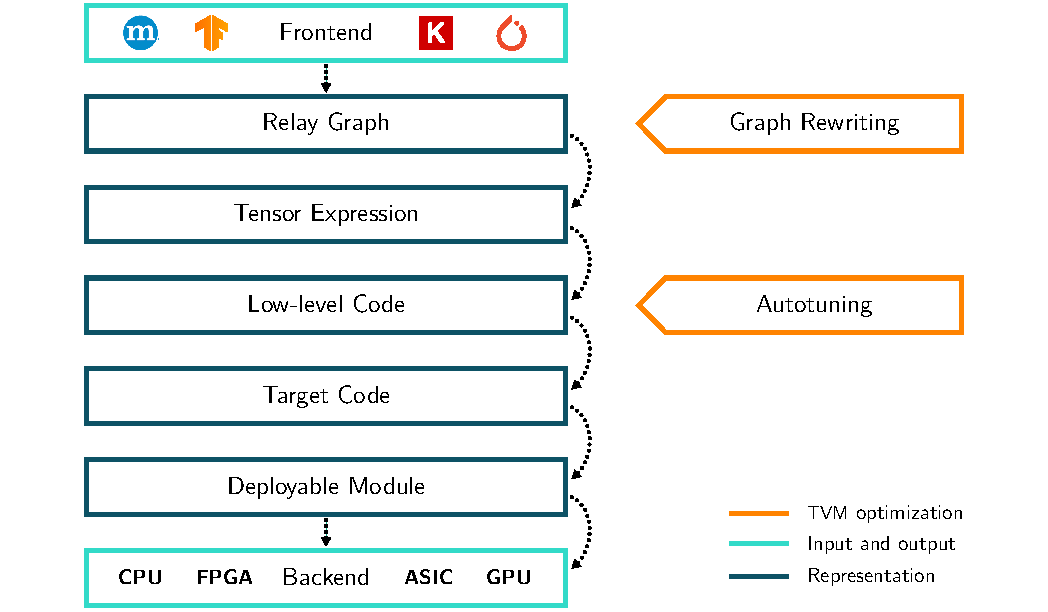
\includegraphics[width=\textwidth]{tvm_stack.pdf}%
	\caption{Levels of abstractions in TVM flow}
	\label{fig:tvm-stack}
\end{figure}

The top layer in the TVM stack is Relay. Relay is an intermediate model representation that enhances traditional computation graphs with concepts of functional programming to form a more powerful language. Relay supports shape-dependent tensor types and automatic differentiation, which is essential for \gls{dl} training~\cite[p.~61]{Roesch.2018}.  Additionally, a runtime to execute Relay programs in various programming languages is provided and needs to be present whenever executing TVM-based models. Relay programs can be created programmatically or from a textual source code. More convenient for users, however, is the import from diverse frontends, including TensorFlow, Keras, PyTorch and MXNet, which enables the use and optimization of existing models. Graph-level optimization in TVM is pass-based, with each pass inspecting or rewriting the syntax tree of the Relay program in some way. Standard passes are provided and perform, for example, automatic differentiation, type inference, operator fusion or tensor layout transformations~\cite[p.~3]{Chen.2018b}. Beyond that, writing custom passes is facilitated by an extensible design.

Next in the stack is a tensor expression language, which has similar features as \gls{tc}'s. It allows user to describe computation rules that generate a tensor without specifying loop structures and other details. The rules are composed of primitive mathematical operations like addition and multiplication and are expressive enough to describe tensor, matrix and vector operations. TVM comes with tensor expressions for common computations used in \gls{dl} such as various activation functions, convolution, pooling, and matrix multiplication~\cite[p.~4~f.]{Chen.2018b}. The tensor expression language is used to describe the functionality of tensor operators from the model. In the usual TVM workflow, the required operators are extracted from the Relay graph and matched with existing tensor expressions, so there is no need to write them manually.

Implicit tensor expressions need to be mapped to explicit, backend-independent loq-level code. TVM, again, uses a pass-based design, which is different from \gls{tc}'s polyhedral approach. Basic transformations called schedule primitives are combined into schedules that are applied to the naïve straightforward implementation to, for example, change loop structures and thread binding. This design is based on the Halide language for image processing, which works with similar multi-dimensional data as \gls{dl}, but enhances it with more primitives to optimize accelerator performance. TVM leverages nested and cooperative parallelism to make effective use of \gls{gpu} memory structure by enabling data reuse across threads through shared memory regions. This is done in a special memory scoping pass. TVM also equips the low-level code with hardware-specific instructions through a tensorization pass which matches computations patterns with a corresponding intrinsic from the target (such as general matrix multiply), making it extensible for new hardware architectures. A latency hiding pass introduces explicit management of fine-grained synchronization for memory and computation instructions on specialized \gls{dl} accelerators~\cite[p.~5~f.]{Chen.2018b}. Default schedule templates are provided for every hardware type, but users can create their own templates to incorporate their knowledge of the backend.

Low-level code cannot be executed, but it can directly be converted to target-specific code and then compiled for the target device. Backend-specific code generators create the source files, which are then built by the respective compiler and packed into a module which contains the implementation of all tensor operators in the model. This module can be deployed along with a JSON description of the Relay graph and a parameter file containing the weights for all operations. The TVM runtime (\SIrange{300}{600}{\kilo\byte}) needs to be installed on the target system to execute the model. However, a full \gls{dl} framework is not required, making TVM modules very lightweight to integrate into applications.

While \glspl{tc}'s autotuner is guided by a genetic algorithm, TVM uses a \gls{ml}-based cost model to predict the performance of an implementation. Specifically, gradient boosted trees are used because of their advantage in training and prediction speed over neural network-based models. Since the model is queried frequently, the inference overhead must be smaller than the profiling it seeks to replace. While profiling can be in the order of seconds, the gradient boosted trees model performs prediction in \SI{0.67}{\milli\second} on average. Model training time also needs to be considered; the cost model is updated periodically as more configurations have been explored, which improves the accuracy for further predictions with more experimental trials. This learning-based approach is preferable to static, predefined cost models for every new hardware target, which is infeasible due to the increasing complexity of modern accelerators~\cite[p.~8~f.]{Chen.2018b}. Pure low-level code cannot be used as input for the cost model, we need to encode it into a vector space first. This encoding needs to be a transferable representation which is invariant between programs to make the cost model effective. Encoding works by extracting context features from each loop level, including memory access count, reuse ratio of each memory buffer and loop annotations such as \enquote{unroll} or \enquote{parallel}. Furthermore, context relation features enable generalization across different loop nest patterns~\cite[p.~4]{Chen.2018}.

\begin{figure}
	\centering
	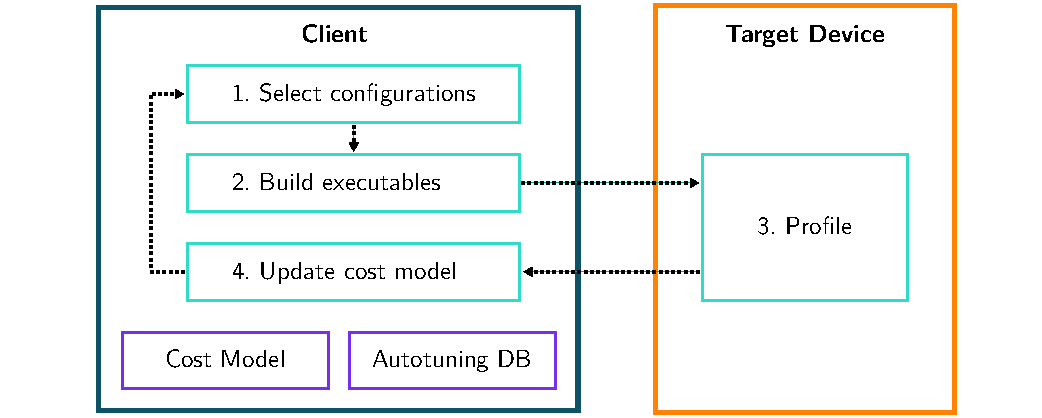
\includegraphics[width=\textwidth]{tvm_autotuning.pdf}%
	\caption{Iterative autotuning process in TVM}
	\label{fig:tvm-autotuning}
\end{figure}

Autotuning in TVM is an iterative process as seen in Figure \ref{fig:tvm-autotuning}. We call the execution of the autotuning process for one model a \textit{job}. The component that executes the autotuning logic for one job the \textit{autotuning client}. Profiling the implementation requires execution on the actual target device. This can make autotuning a distributed process, if the client is another device. However, autotuning is not performed for a whole model at once, but rather for a set of \textit{tasks} which correspond to autotunable tensor operators with a specific configuration (shapes, padding stride). These tasks need to be extracted from the model before starting the process for each of them. Autotuning consists of four stages that depend on each other, making it necessary to execute them in sequential order. Understanding the stages and their dependencies is key for enabling large-scale autotuning.

\begin{description}
	\item[Initialization] At the start of each task, profiling results from previous jobs are loaded from a global autotuning database, a file that contains data from all previous jobs along with information about the target and configuration. The loaded results are passed to the cost model for transfer learning. This yields good cost model from the beginning and improve in quality over time. Then the autotuning loop can be launched.
	\item[1. Select candidate configurations] At the start of each iteration, a batch of candidate configurations that have a promising performance is selected using the cost model. A simple strategy such as enumerating and running every configuration through the model, then selecting the top performers is impracticable with large search spaces. Rather, candidates are selected using parallel simulated annealing, which is a heuristic optimization algorithm that trades off finding an exact optimum for a much improved speed. Additionally, exploration is ensured by random selection of some configurations. If no training data exist yet, random candidates are picked.\footnote{In TVM's implementation, the selection of the next candidates is actually performed at the end of the iteration after updating the model, and the first stage just picks a batch from the already selected configurations. However, it is more logically simpler to think of the candidate selection using simulated annealing as part of the first stage. Furthermore, it is not wrong due to the iterative nature of autotuning.}
	\item[2. Build executables] The client combines the batch of configurations from the previous stage with the schedule template, then applies the schedule to the tensor expression for the operator of the current task. The resulting low-level code is then translated into backend-specific code and compiled. In case the target hardware is different from the client hardware, cross-compilation is necessary. The result is a tar file that contains everything that is necessary to run the executable, namely the compiled tensor operator itself and backend-specific code such as the CUDA driver library for NVIDIA \glspl{gpu}.
	\item[3. Profile on target device] Since the cost model's prediction of the implementation's performance are not completely reliable, the real performance needs to be evaluated on the target device. The tar files from the build stage are uploaded to the target device. Then the implementation is profiled by running the executable a number of times with random data. The measured execution times are averaged and returned to the client, which stores the results in the autotuning database for this job.
	. Parallel profiling on the same computation resource should be avoided to guarantee accurate results.
	\item[4. Update cost model] The cost model is updated with the measurements from the profiling stage to improve the proposed configurations in the next iteration. This is only done after a sufficient number of new profiling data has been collected, so this stage might be skipped in some iterations.
	\item[Finalization] After a certain number of trials, the loop is stopped. The best configuration that was discovered can now be used to build a faster implementation of the tensor operator that was optimized. Usually, the best configuration is also written into a separate database that contains only the best known configurations. The autotuning database for this job is merged with the global one. This concludes the autotuning process in TVM.
\end{description}

The target device is usually specialized for \gls{dl} workloads. Therefore, it is desirable to run the client on a machine that features a strong CPU to accelerate the compute-intensive build and profile stages. This distribution across multiple machines requires an \gls{rpc} infrastructure that makes it possible to profile on a different server. TVM's \gls{rpc} architecture (Figure \ref{fig:tvm-rpc}) comprises three components:
\begin{description}
	\item[Client] A client runs an autotuning job and and is responsible for selecting the candidate configurations, building the executables and updating the model with the profiling results. This means that the client contains both the cost model and the autotuning database. It also controls the profiling, but the actual execution is happening on servers.
	\item[Server] A server can receive and execute TVM modules, which basically makes it an RPC-enabled TVM runtime that runs on the target device. The interface on the client side does not change because TVM transparently handles remote execution like local execution. A server has a \textit{device key}, which is an arbitrary identifier for a certain device type, but usually is it based on the accelerator's name. Multiple servers can have the same device key if they run on identical target devices.
	\item[Tracker] A tracker keeps a list of servers to help clients discover unused servers for profiling. The tracker matches incoming requests from clients with free servers using a FIFO-based scheduling algorithm. Scheduling is implemented using a queue for servers and a heap for requests. Requests can have a priority.
\end{description}
TVM's \gls{rpc} is enabled by two distinct protocols. The control plane protocol is used for communication involving the tracker, namely server registration and requests from clients. The data plane protocol facilitates remote execution on a server and is initiated by clients.

\begin{figure}
	\centering
	
\includegraphics[width=\textwidth]{tvm_rpc.pdf}%
	\caption{TVM's RPC architecture}
	\label{fig:tvm-rpc}
\end{figure}

First, the tracker is started and listens on the first free port between 9190 and 9199. Then, one or multiple servers are started which bind to ports between 9091 and 9199. They register with the tracker by transmitting the device key, and the address and port which clients can use to connect. The tracker puts them in a queue, with separate queues for every device key. At this point, clients can request a server with a specific device key. The tracker matches the free server with that device key that registered first with the request that has the highest priority, then the one that was received first. If requests have the same priority, scheduling degrades to simple FIFO scheduling, and the request heap effectively becomes a queue. Once a client has acquired a server, it is marked as busy in the tracker and the client initiates a connection to the server to use its TVM runtime for profiling.

Since autotuning works in batches, usually not a single but multiple servers are requested to run profiling in parallel. This can speed up profiling if multiple target devices are available. For example, if a machine is equipped with 4 \glspl{gpu} of the target device type, 4 RPC servers can be launched on that machine, with each one being assigned to a different one of the \glspl{gpu}.

In this project, we use TVM instead of \gls{tc} because of the novel, machine learning-based approach, which promises better results than a genetic algorithm due to better guidance by the cost model. We are using the TVM version from June 11, 2019 (commit \href{https://github.com/dmlc/tvm/tree/8f219b9}{8f219b9}) for comparable results throughout the project. We made some modifications:
\begin{itemize}
	\item Add decomposed version of autotuner with separate methods for stages
	\item Add time measurement for autotuning stages
	\item Add loading of autotuning records from multiple files
	\item Fix Tensorflow import for models including PlaceholderWithDefault
\end{itemize}
